\providecommand{\tightlist}{%
  \setlength{\itemsep}{0pt}\setlength{\parskip}{0pt}}\documentclass{article} 
\usepackage{hyperref}
\usepackage[T1]{fontenc}
\usepackage{framed,graphicx,xcolor}
\usepackage{listings}

\graphicspath{ {images} }

\begin{document}

\hypertarget{detektor-kart}{%
\section{Detektor Kart}\label{detektor-kart}}

\hypertarget{problem}{%
\subsection{Problem}\label{problem}}

Klasyfikacja kart z obrazu strumieniowanego. Rozwiązanie powinno w
czasie rzeczywistym określać kolor i wartość zaprezentowanych kart.
Dodatkowo algorytm powinien rozpoznawać dowolną ilość znajdujących się
na ekranie / strumieniu kart.

\hypertarget{rozwiux105zanie}{%
\subsection{Rozwiązanie}\label{rozwiux105zanie}}

Proponowany algorytm porównuje aktualnie odnalezioną wartość i kolor,
dla każdej znalezionej na obrazie karty, z wartością z bazy posiadanych
kolorów i wartości. W bazie przechowywane są odpowiednio przygotowane
zdjęcia cech kart. Obraz, który zostanie najlepiej dopasowany - będzie
posiadał najmniej niedopasowanych pixeli i przekroczy pewną wartość
progową zostanie uznany za poprawny a karta rozpoznana.

\hypertarget{narzux119dzia}{%
\subsubsection{Narzędzia}\label{narzux119dzia}}

\begin{itemize}
\tightlist
\item
  Python 3.6.8
\item
  OpenCV 2
\item
  NumPy
\end{itemize}

\hypertarget{ux15brodowisko-uruchomieniowe}{%
\subsubsection{Środowisko
uruchomieniowe}\label{ux15brodowisko-uruchomieniowe}}

\begin{itemize}
\tightlist
\item
  \textbf{OS}: Linux - Debian Wheezy
\item
  \textbf{Platforma}: RaspberryPi 3B
\item
  \textbf{Kamera}: PiCamera - lub substytut działający z modułem
  PiCamera
\end{itemize}

\hypertarget{skruxf3cony-algorytm-dziaux142ania}{%
\subsubsection{Skrócony algorytm
działania}\label{skruxf3cony-algorytm-dziaux142ania}}

\begin{lstlisting}[language=Python]
for frame in stram:
    cards = detect_all_cards_present()
    for card in cards:
        rank_part, suite_part = zoom_card(card)
        rank_diff, rank = match_rank(rank_part)
        suite_diff, suite = match_suite(suite_part)
        if rank_diff < RANK_THRESH and suite_diff < SUITE_THRESH:
            make_an_overlay_on_card(card=card, rank=rank, suite=suite)
\end{lstlisting}

\hypertarget{kroki-dziaux142ania-algorytmu}{%
\subsubsection{Kroki działania
algorytmu}\label{kroki-dziaux142ania-algorytmu}}

\hypertarget{pobranie-obrazu-z-kamery}{%
\paragraph{1. Pobranie obrazu z kamery}\label{pobranie-obrazu-z-kamery}}

Całkowite wymiary pobieranego obrazu to 1280x720 pixeli. Jest to
spowodowane dobrą proporcją mocy obliczeniowej potrzebnej do analizy
takiego obrazu a samą jakością obrazu.

\begin{figure}
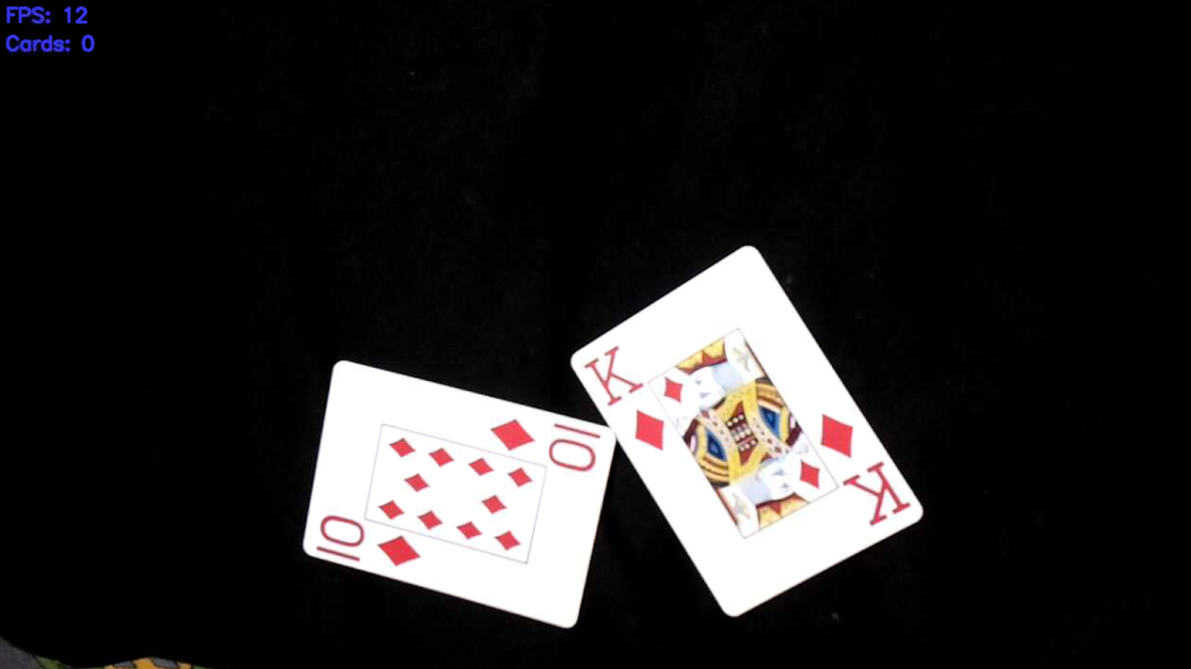
\includegraphics[scale=0.4]{/home/piotr/Documents/python/kck/card-detector/docs/images/step1.png}
\centering
\end{figure}

\hypertarget{wydzielenie-kart-z-obrazu}{%
\paragraph{2. Wydzielenie kart z
obrazu}\label{wydzielenie-kart-z-obrazu}}

Wydzielanie poszczególnych kart odbywa się na zasadzie wyszarzania,
rozmazywanie i thresholdingu obrazu pobranego w poprzednim kroku.
Wartość porogowa podczas thresholdingu jest ustalana dynamicznie na
podstawie środkowego piksela w najwyższym rzędzie obrazu. Następnie za
pomocą funkcji wbudowanych w bibliotekę OpenCV wyznaczany jest obwód
poszczególnych kart. Każdy wykryty obwód jest sprawdzany pod kątem
ilości posiadanych narożników (conajmniej 4) i zajmowanego pola.
Pozytywne przejście testów sprawia, że analizowany obwód jest
akceptowany jako karta.

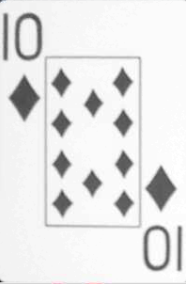
\includegraphics{/home/piotr/Documents/python/kck/card-detector/docs/images/step2.png}
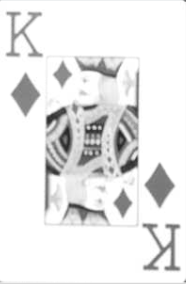
\includegraphics{/home/piotr/Documents/python/kck/card-detector/docs/images/step22.png}

\hypertarget{wydzielenie-koloru-i-wartoux15bci-karty}{%
\paragraph{3. Wydzielenie koloru i wartości
karty}\label{wydzielenie-koloru-i-wartoux15bci-karty}}

Ze względu na właściwość kart do gry jaką jest stałe miejsce
występowania wartości i koloru niezależnie od orientacji karty - góra,
dół - operacja wydzielania cech karty jest łatwa. Wystarczy tylko wyciąć
z obrazu karty jej odpowiedni kawałek, tj. lewy górny narożnik.
Następnie należy porównać go z bazą dostępnych kolorów i wartości.


\includegraphics{/home/piotr/Documents/python/kck/card-detector/docs/images/step31.png} 

\includegraphics{/home/piotr/Documents/python/kck/card-detector/docs/images/step35.png}

\includegraphics{/home/piotr/Documents/python/kck/card-detector/docs/images/step33.png}

\hypertarget{naux142oux17cenie-rezultatuxf3w-klasyfikacji-na-obraz-wyjux15bciowy}{%
\paragraph{4. Nałożenie rezultatów klasyfikacji na obraz
wyjściowy}\label{naux142oux17cenie-rezultatuxf3w-klasyfikacji-na-obraz-wyjux15bciowy}}

Jest to tylko jeden z proponowanych sposobów prezentacji wyników, w
którym nazwy rozpoznanych kart są nakładane na same karty, a informacja
jest uzupełniana o stopień pewności. Dodatkowo informacje są kodowane
kolorami na podstawie stopnia pewności.

\hypertarget{wyniki-dziaux142ania-algorytmu}{%
\subsection{Wyniki działania
algorytmu}\label{wyniki-dziaux142ania-algorytmu}}

\hypertarget{jedna-karta}{%
\subsubsection{Jedna karta}\label{jedna-karta}}

W przypadku pojedynczych kart prezentowany algorytm działa z blisko
100\% skutecznością, rozpoznając karty we wszystkich prezentowanych
przypadkach

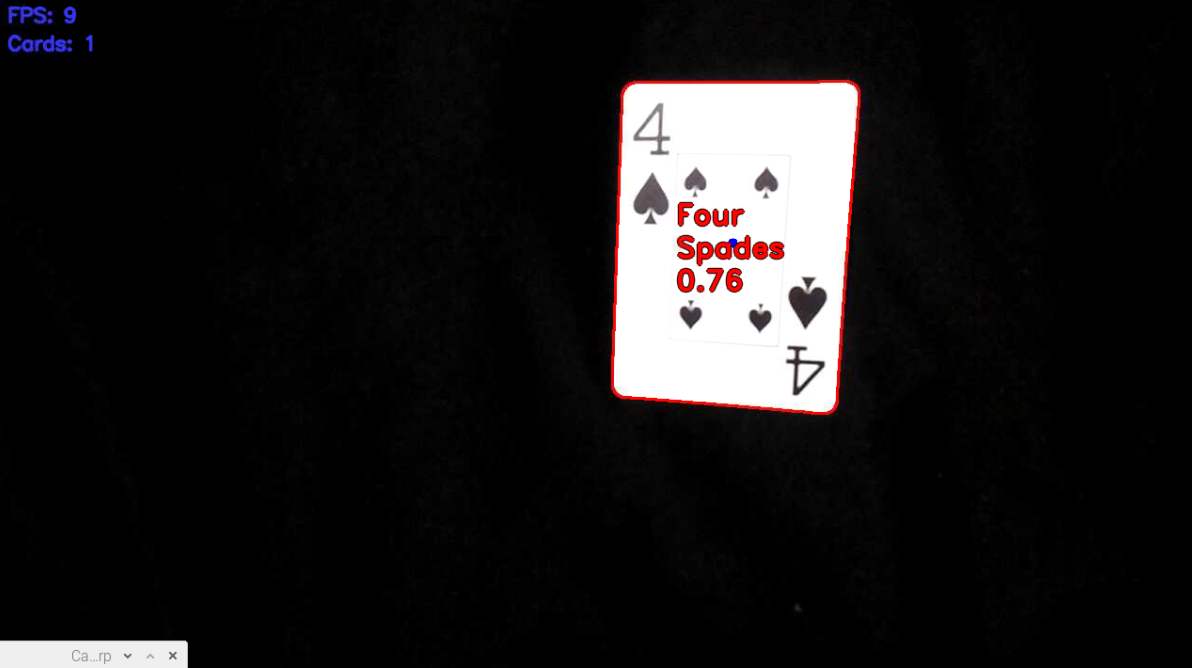
\includegraphics[scale=0.4]{/home/piotr/Documents/python/kck/card-detector/docs/images/one_1.png}
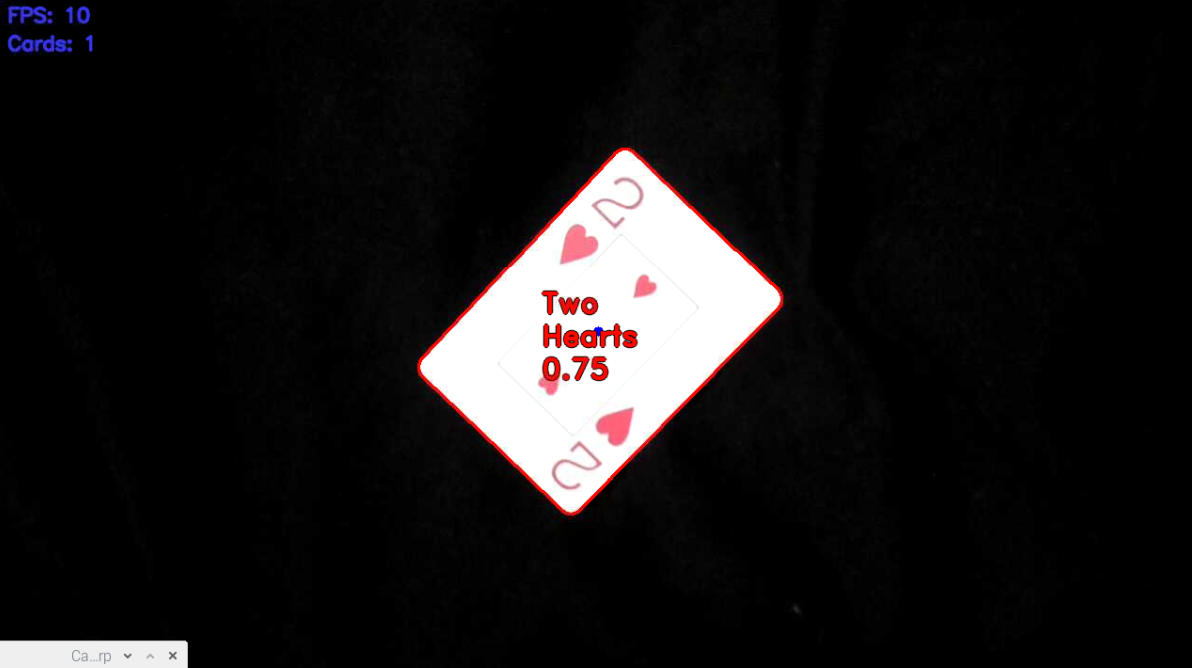
\includegraphics[scale=0.4]{/home/piotr/Documents/python/kck/card-detector/docs/images/one_2.png}
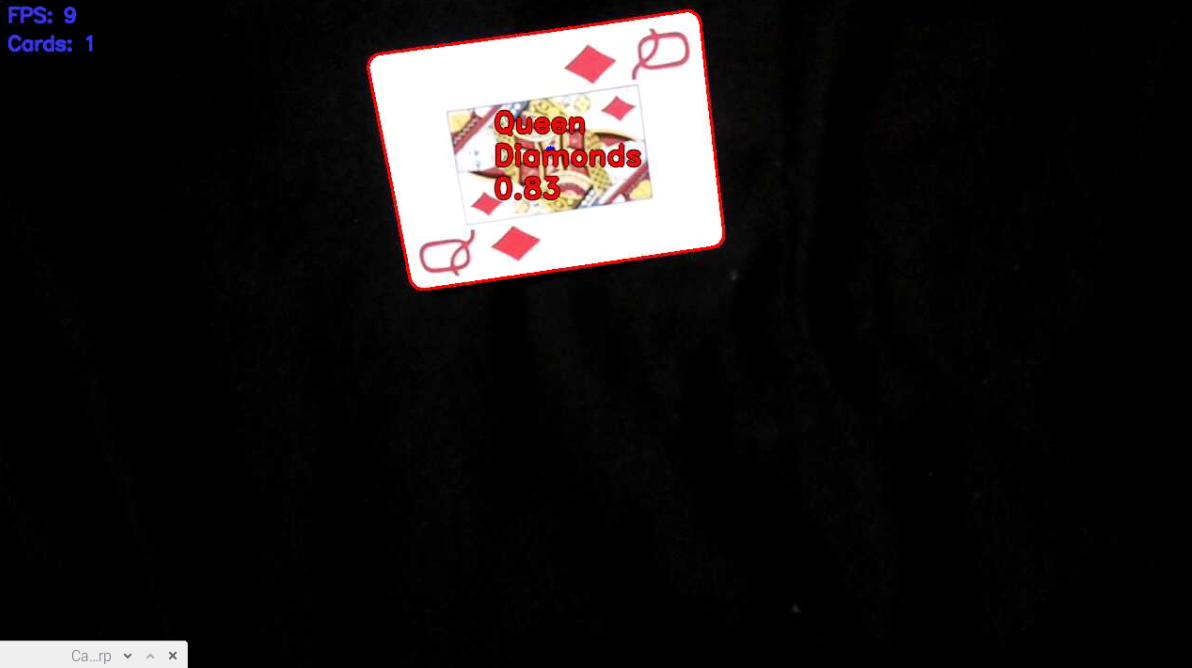
\includegraphics[scale=0.4]{/home/piotr/Documents/python/kck/card-detector/docs/images/one_3.png} 
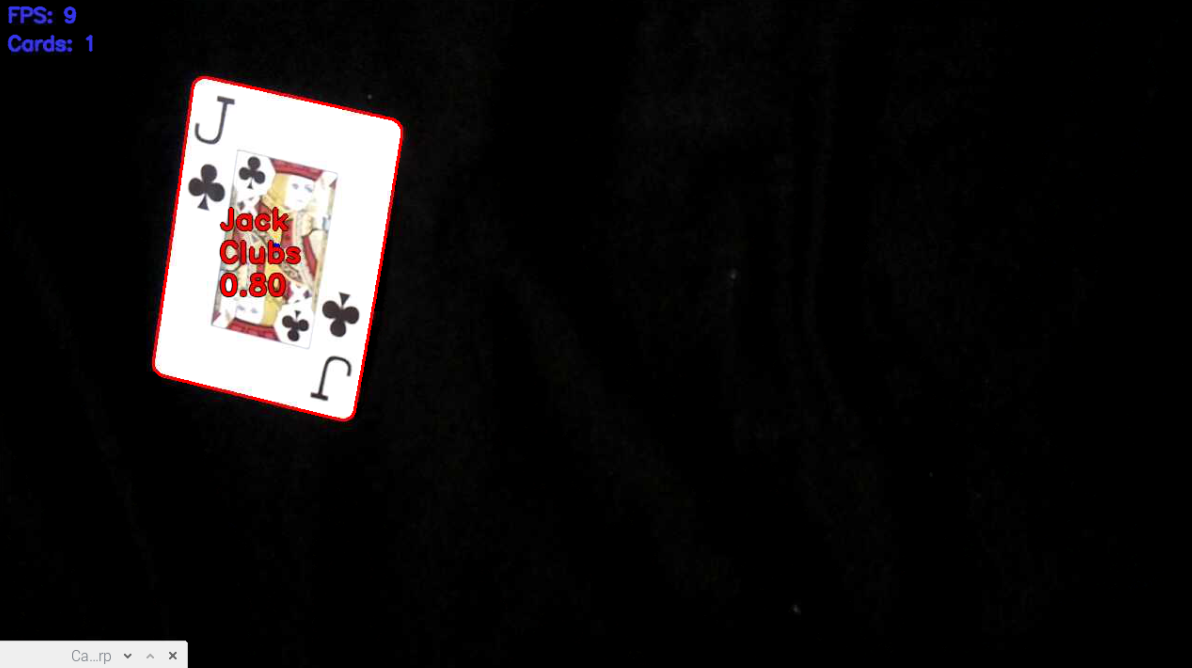
\includegraphics[scale=0.4]{/home/piotr/Documents/python/kck/card-detector/docs/images/one_4.png}

\hypertarget{dwie-karty}{%
\subsubsection{Dwie karty}\label{dwie-karty}}

Tak jak w przypadku pojednyczych kart algorytm radzi sobie bardzo
dobrze. Problematyczne natomiast są sytuacje, w których karty nachodzą
na siebie.

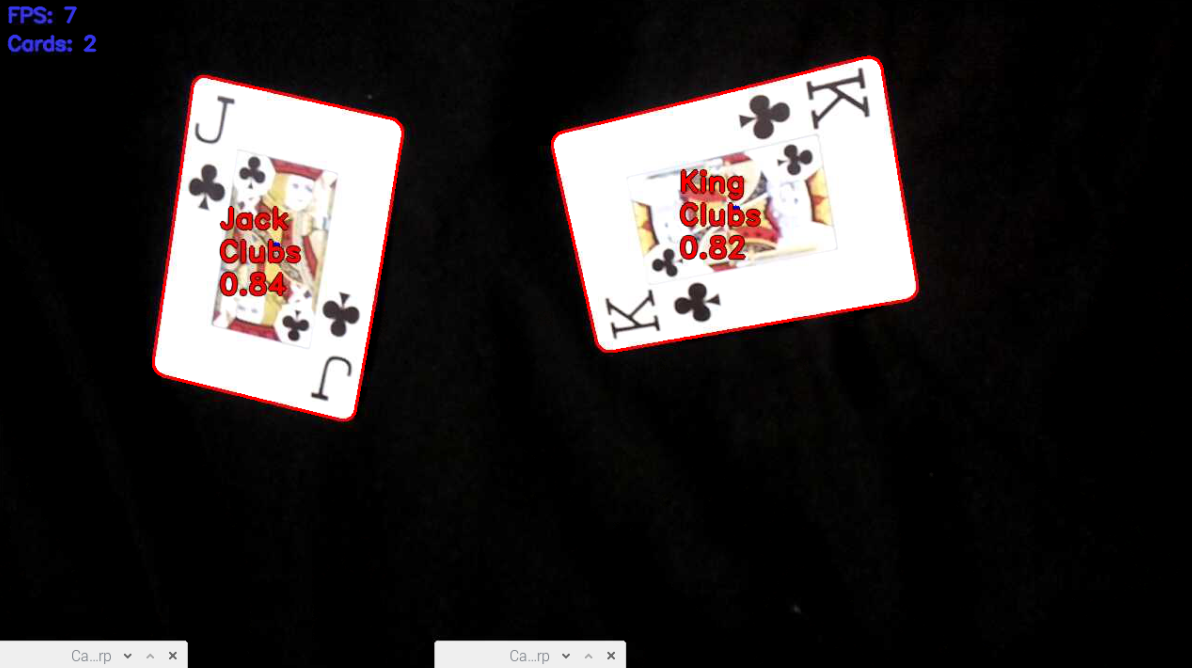
\includegraphics[scale=0.4]{/home/piotr/Documents/python/kck/card-detector/docs/images/two_1.png} 
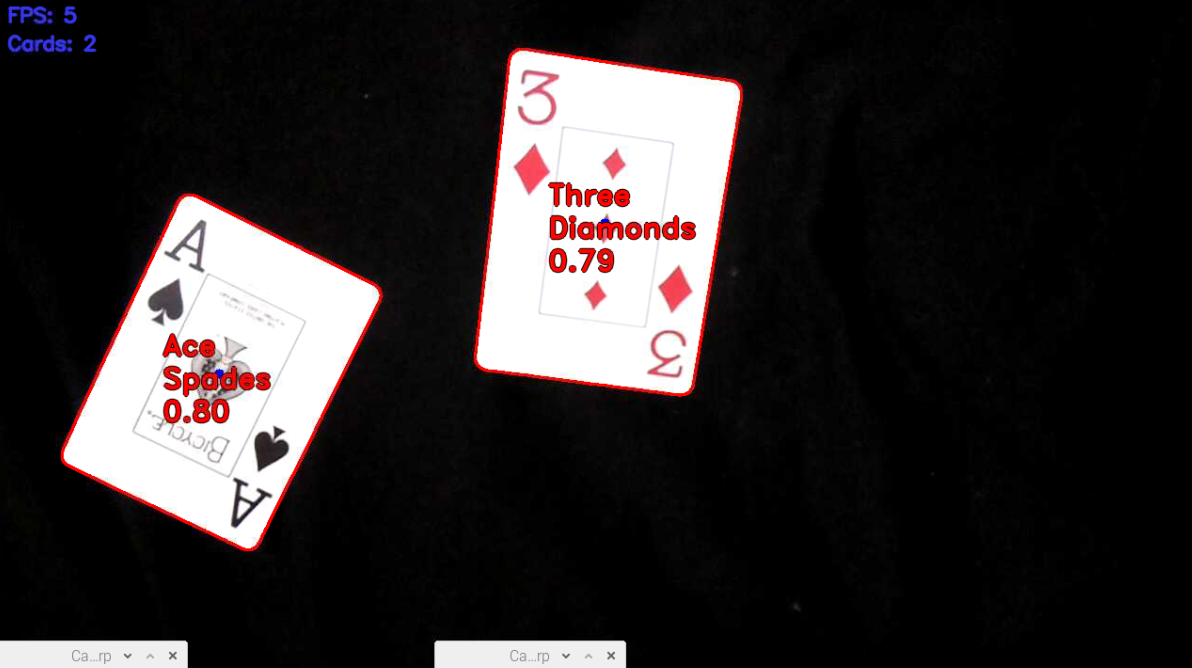
\includegraphics[scale=0.4]{/home/piotr/Documents/python/kck/card-detector/docs/images/two_2.png}
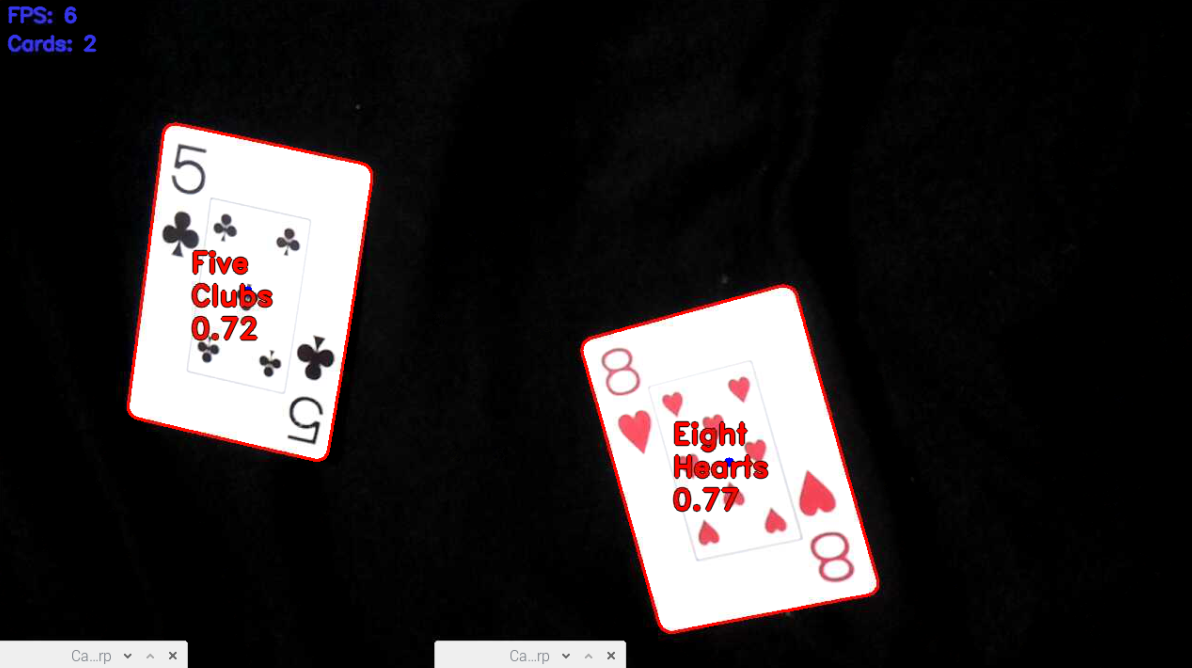
\includegraphics[scale=0.4]{/home/piotr/Documents/python/kck/card-detector/docs/images/two_3.png} 
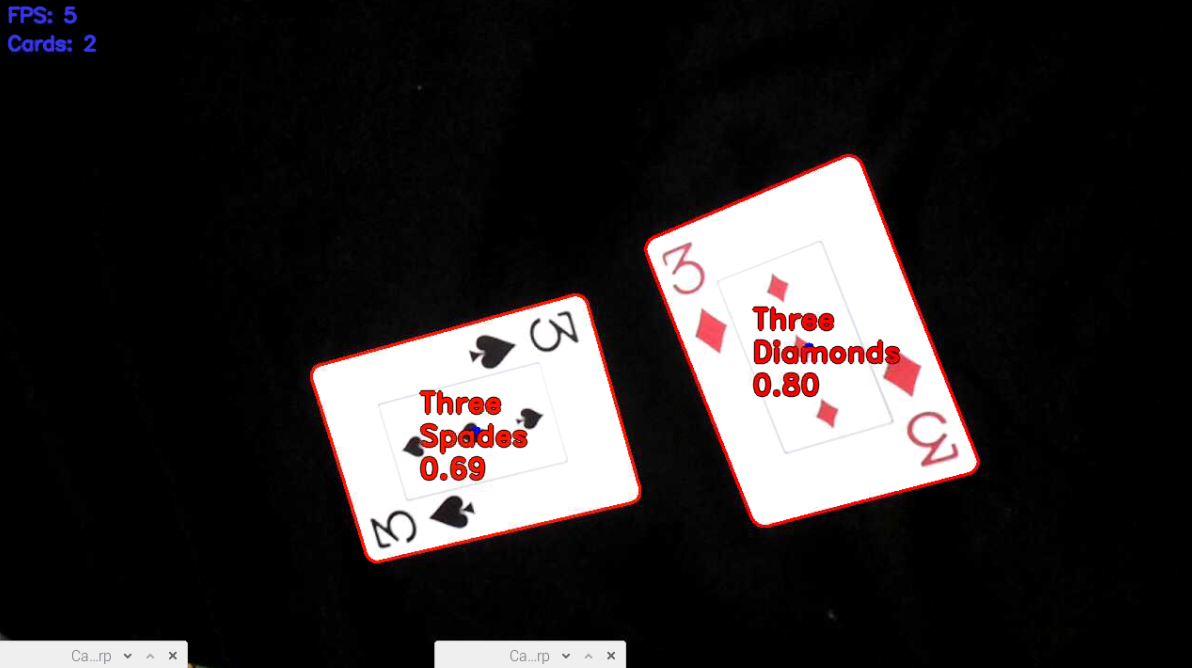
\includegraphics[scale=0.4]{/home/piotr/Documents/python/kck/card-detector/docs/images/two_4.png}

\hypertarget{trzy-i-wiux119cej-kart}{%
\subsubsection{Trzy i więcej kart}\label{trzy-i-wiux119cej-kart}}

Tak jak w przypadku dwóch kart algorytm wykazuje wysoką efektywność, o
ile karty nie nachodzą na siebie.

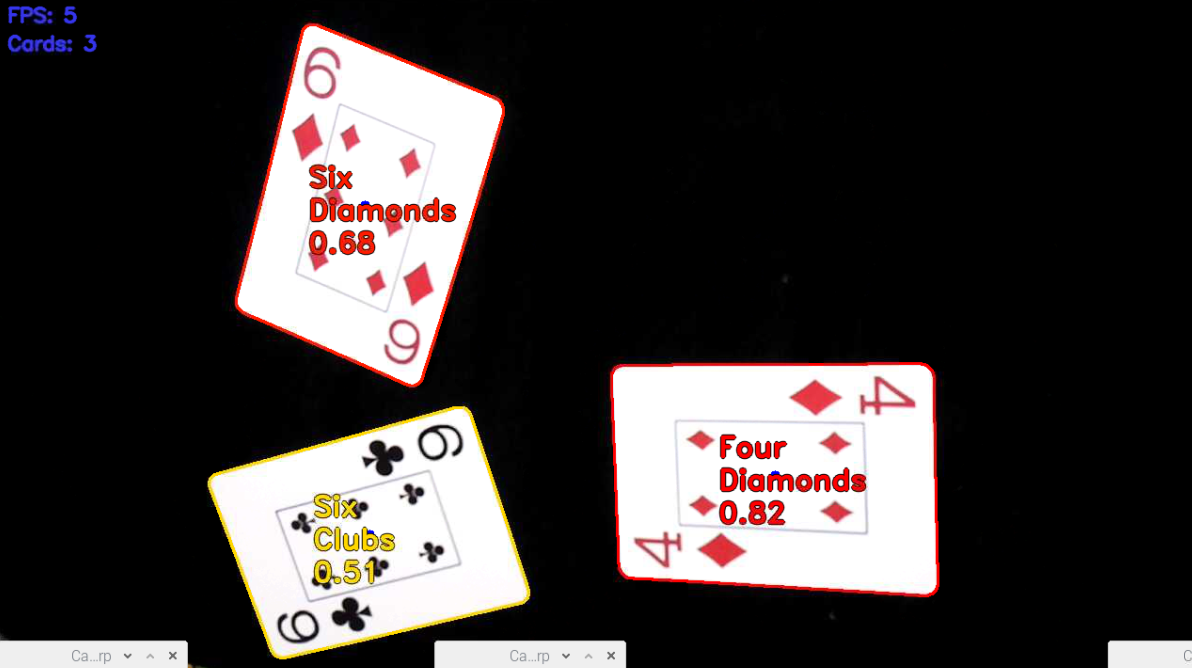
\includegraphics[scale=0.4]{/home/piotr/Documents/python/kck/card-detector/docs/images/three_1.png}
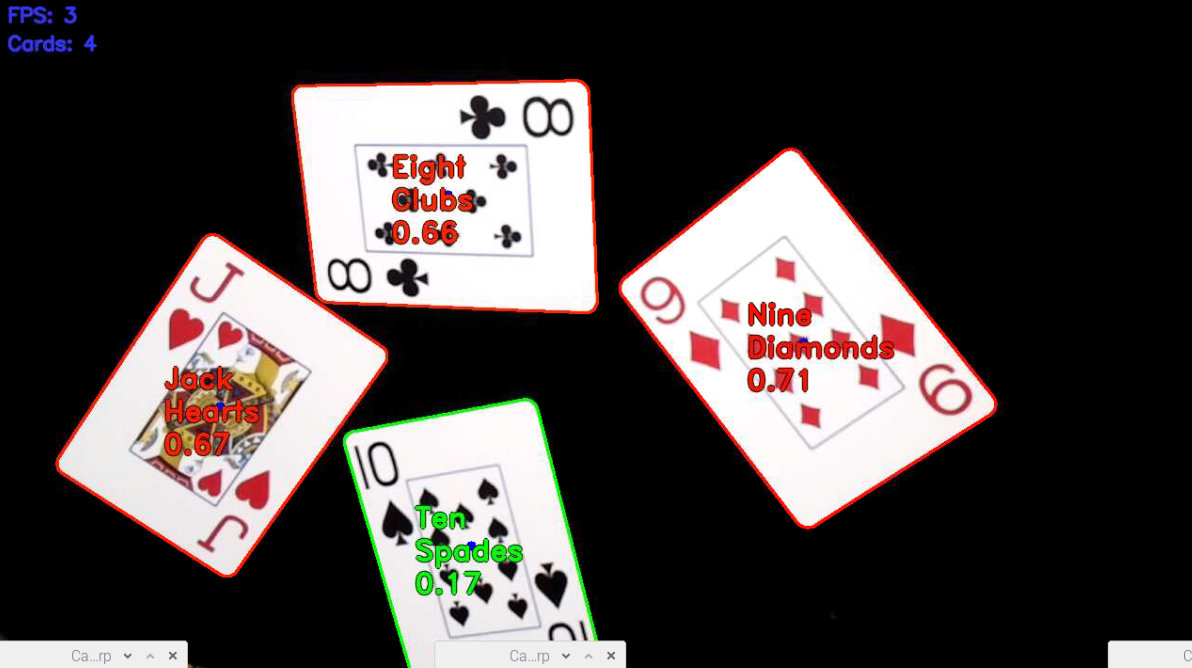
\includegraphics[scale=0.4]{/home/piotr/Documents/python/kck/card-detector/docs/images/three_2.png}
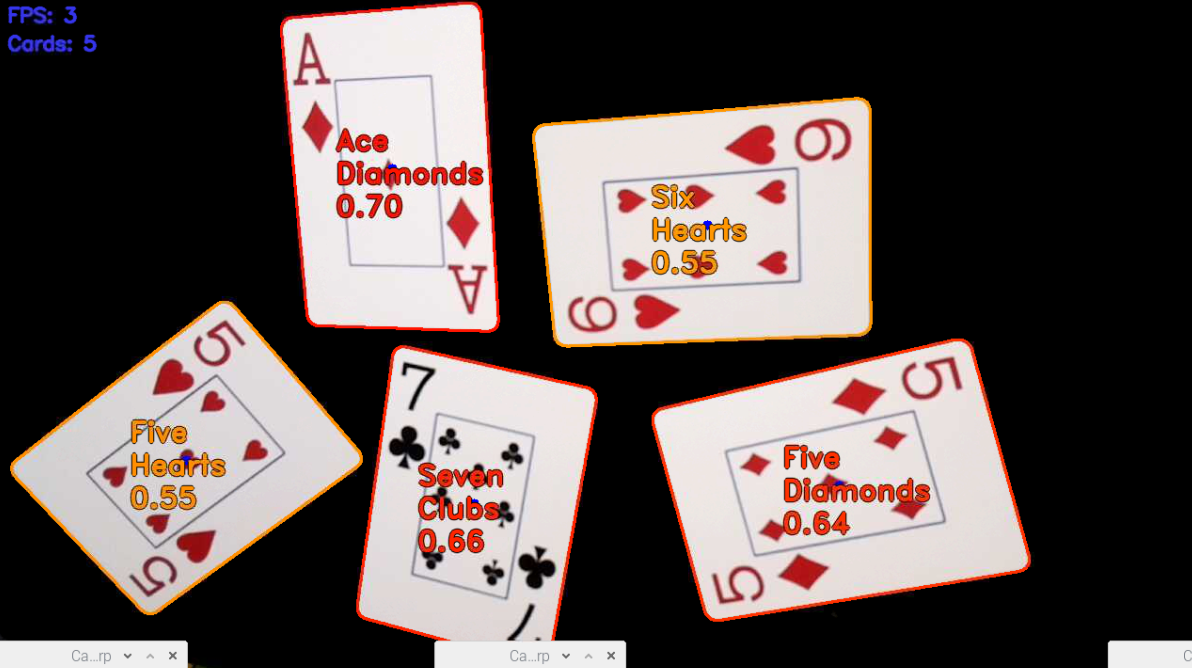
\includegraphics[scale=0.4]{/home/piotr/Documents/python/kck/card-detector/docs/images/three_3.png}
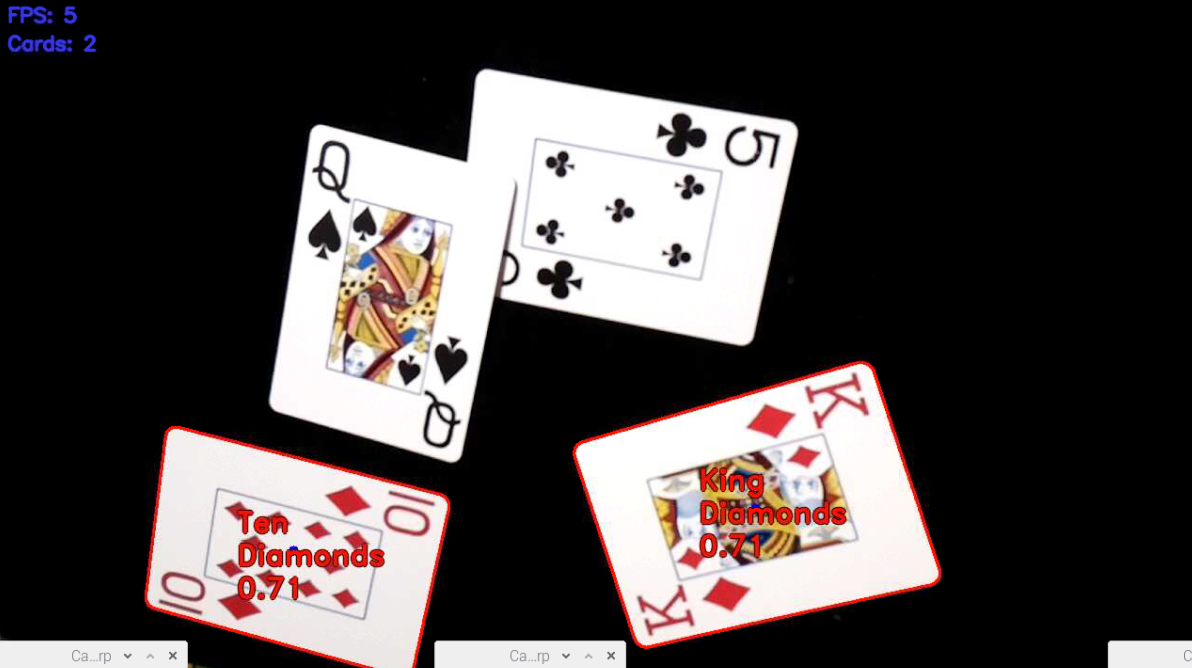
\includegraphics[scale=0.4]{/home/piotr/Documents/python/kck/card-detector/docs/images/three_4.png}

\hypertarget{podsumowanie}{%
\subsection{Podsumowanie}\label{podsumowanie}}

\hypertarget{komentarz-do-wynikuxf3w}{%
\subsubsection{Komentarz do wyników}\label{komentarz-do-wynikuxf3w}}

Na podstawie wyżej zaprezentowanych wyników, stwierdzam, że algorytm
cechuje się wysoką efektywnością w rozpoznawaniu kart. W szczególności
efektywności tej nie zmniejszają zmieniające się warunki świetlne o ile
nie tworzą silnych refleksów powodujących efekt olśnienia kamery.
Dodatkowo na wyniki nie ma wpływu ułożenie i orientacja kart a także ich
ilość.

Znaczący wpływ na jakość klasyfikacji ma nakładanie się kart na siebie.
W takich przypadkach nie jest możliwe szybkie poprawne rozpoznanie kart.
Jest to spowodowane błędnym wykrywaniem obwodu kart znajdujących się na
stole, a co za tym idzie obydwie karty są wykrywane jako jedna. Sprawia
to, że algorytm wydzielający karty z obrazu odrzuca je, ponieważ ich
łączna powierzchnia jest znacząco większa od maksymalnej akceptowalnej
powierzchni karty.

\hypertarget{dalszy-rozwuxf3j}{%
\subsubsection{Dalszy rozwój}\label{dalszy-rozwuxf3j}}

Elementem wymagającym dalszych prac jest moduł separacji poszczególnych
kart z obrazu. W szczególności polepszenie mechanizmu pozwalającego na
oddzielania nachodzących na siebie kart. Implementacja nie jest trudna z
punktu matematycznego, ponieważ wystarczy określić conajmniej dwa
przeciwległe narożniki a wszystkie pozostałe można przybliżyć.
Problematycznym natomiast może okazać się czas potrzeby na wykonanie
wszystkich obliczeń związanych z przybliżaniem brakujących narożników.
Zauważmy, że algorytm dokonuje analizy obrazu w czasie rzeczywistym i
niedopuszczalne jest wykonywanie obliczeń zajmujących duże ilości czasu.
Jest to ważne nie tylko ze względów estetycznych - ilość klatek na
sekundę - ale i ze względów praktycznych zastosowań algorytmu. Długi
czas przetwarzania sprawia, że szybko poruszające się karty mogą nie być
wykryte, ponieważ zdążą przelecieć przed polem widzenia kamery w czasie
kiedy algorytm będzie analizował poprzednią klatkę i nie zdąży
zarejestrować klatki z lecącą kartą. Jest to gółwny powód dlaczego w
prezentowanym rozwiązaniu bazującym na platformie RaspberryPi nie
zaimplementowano wyżej wspomnianej poprawki.

\end{document}